% Charlotte Geiger - Manuel Lippert - Leonard Schatt
% Physikalisches Praktikum

% Main-Datei für die Auswertung in TeX

% Struktur:
% Für jeden Abschnitt gibt es einen Ordner, damit jeder individuell an seinen Aufgaben arbeiten
% kann, ohne beim merge in GitHub Konflikte zu erhalten. Deshalb werden alle Unteraufgaben auch 
% extra in Ordner angelegt. Die einzelnen Dateien über den input Befehl einfügbar.
% Bilder und andere Grafik werden im Ordner Grafik abgelegt 


% Packages
\documentclass[paper=a4,bibliography=totoc,BCOR=10mm,twoside,numbers=noenddot,fontsize=11pt]{scrreprt}
\usepackage[ngerman]{babel}
\usepackage[T1]{fontenc}
\usepackage[latin1, utf8]{inputenc}
\usepackage{lmodern}
\usepackage{graphicx}
\usepackage{nicefrac}
\usepackage{fancyvrb}
\usepackage{amsmath,amssymb,amstext}
\usepackage{siunitx}
\usepackage{url}
\usepackage{natbib}
\usepackage{microtype}
\usepackage[format=plain]{caption}
\usepackage{physics}

% Zusätzliche Packages
\usepackage{geometry}
\usepackage{anyfontsize}
\usepackage{xcolor}
\usepackage{ifthen}
\usepackage[scaled]{uarial}
\usepackage[absolute,overlay]{textpos}
\usepackage{amsfonts}
\usepackage{xstring}
\usepackage{tikz}
\usepackage{pdfpages}

% Abschnittseinrückung und -abstand
% Die folgenden Zeilen sollen möglichst nicht verändert werden
\parindent 0.0cm
\parskip 0.8ex plus 0.5ex minus 0.5ex

% Anzahl und Größe von Gleitobjekten
% maximal 2 Objekte oben und unten
% erlaubt auch größere Bilder, welche die ganze Seite benötigen
% Die folgenden Zeilen sollen möglichst nicht verändert werden
\setcounter{bottomnumber}{2}
\setcounter{topnumber}{2}
\renewcommand{\bottomfraction}{1.}
\renewcommand{\topfraction}{1.}
\renewcommand{\textfraction}{0.}

%\sc und \bc veraltet. Daher: (20.09.2018)
\DeclareOldFontCommand{\sc}{\normalfont\scshape}{\@nomath\sc}
\DeclareOldFontCommand{\bf}{\normalfont\scshape}{\textbf}

% Verschiedenes
\pagestyle{headings}          % Der Seitenstil sollte möglichst nicht verändert werden
\graphicspath{{./bilder/}}    % Der Pfad für die Abbildungen Abbildungen wird gesetzt
\VerbatimFootnotes            % \verb etc. auch in \footnotes mφglich

\begin{document}

    \nonfrenchspacing

    % 0. Kapitel Cover
    % 0. Cover

% Hier sind nur die Variablen und der Abschnitt Informationen (unten) zu bearbeiten der REst läuft automatisch ab (z.b Farbenänderung)

% Noch abänderbar nur ein Vorschlag
\newgeometry{top=30mm, bottom=20mm, inner=20mm, outer=20mm}
\thispagestyle{empty}

% Colors (Notability Colors)
\definecolor{Notablue}{HTML}{3498DB}		
\definecolor{Notared}{HTML}{CF366C}			
\definecolor{Notagreen}{HTML}{19B092}		
\definecolor{Notaorange}{HTML}{FA9D00}		
\definecolor{Notagrey}{HTML}{969696}		
\definecolor{Notalavendel}{HTML}{9DBBD8}	

% Boolean by default false. Für Absatz in der Überschrift
\newboolean{twoRows}
\newboolean{symbol}

% Funktions
\makeatletter
   \def\vhrulefill#1{\leavevmode\leaders\hrule\@height#1\hfill \kern\z@}
\makeatother
\newcommand*\ruleline[1]{\par\noindent\raisebox{.8ex}{\makebox[\linewidth]{\vhrulefill{\linethickness}\hspace{1ex}\raisebox{-.8ex}{#1}\hspace{1ex}\vhrulefill{\linethickness}}}}

% Variables
\def\schriftgrosse{70}
\def\linethickness{1,5pt}

\def\farbe{black}
\def\fach{PPBphys2}
\def\name{Manuel Lippert - Paul Schwanitz}
\def\titel{Rasterelektronen- \\[0,5cm] mikroskop} % Absatz mit \\[0,5cm]; u = Übung, k = Klausur; s = Skript, e = Ergebnis
\def\bottom{WS2021/22}
\def\datum{13.09.2021}
\def\platz{NWII | 2.1.00.267}
\def\betreuer{Inga Elvers}

\def\teilnehmerm{Manuel Lippert}
\def\emailm{Manuel.Lippert@uni-bayreuth.de}
\def\teilnehmerp{Paul Schwanitz}
\def\emailp{Paul.Schwanitz@uni-bayreuth.de}

%\def\auswertp{}
%\def\messp{}
%\def\protop{}

\def\groupnr{11}

\begin{titlepage}
			
	\centering
	{\LARGE \sffamily {\textbf{\bottom}\par}}
	\vspace{2,5cm}
    {\fontsize{30}{0}\sffamily\ruleline{\textcolor{\farbe}{\textbf{\fach}}}\par}
    \vspace{6cm}
	{\Large\sffamily \ruleline{\name}\par}
		
	\IfSubStr {\titel} {\\[0,5cm]} {\setboolean{twoRows}{true}} {\setboolean{twoRows}{false}}
	
	\ifthenelse{\boolean{twoRows}}
		{
			\begin{textblock*}{21cm}(0cm,8cm) % {block width} (coords), centered		
				{\fontsize{\schriftgrosse}{0}\sffamily\textcolor{\farbe}{\textbf{\titel}}\par}
			\end{textblock*}
		}
		{
			\begin{textblock*}{21cm}(0cm,9cm) % {block width} (coords), centered		
				{\fontsize{\schriftgrosse}{0}\sffamily\textcolor{\farbe}{\textbf{\titel}}\par}
			\end{textblock*} 
		}
	
	% Choose Logo
	\ifthenelse {\equal{\farbe}{Notared}} {\def\logo{Bilder/Logo/UniBTNotared}}
		{\ifthenelse {\equal{\farbe}{Notagreen}} {\def\logo{Bilder/Logo/UniBTNotagreen}}
			{\ifthenelse {\equal{\farbe}{Notablue}} {\def\logo{Bilder/Logo/UniBTNotablue}}
				{\ifthenelse {\equal{\farbe}{Notaorange}} {\def\logo{Bilder/Logo/UniBTNotaorange}}
					{\ifthenelse {\equal{\farbe}{Notagrey}} {\def\logo{Bilder/Logo/UniBTNotagrey}}
						{\ifthenelse {\equal{\farbe}{Notalavendel}} {\def\logo{Bilder/Logo/UniBTNotalavendel}}	
							{\ifthenelse {\equal{\farbe}{black}} {\def\logo{Bilder/Logo/UniBT}}	
								{\def\logo{noLogo}}
							}
						}
					}
				}
			}
		}	

	\IfSubStr{\logo}{noLogo}{\setboolean{symbol}{false}}{\setboolean{symbol}{true}}
	
	% Gruppe
	\vspace{10cm}
	{\large\sffamily{Gruppe \groupnr}}
	
	%Logo
	\vfill

	\ifthenelse{\boolean{symbol}}
		{
			\begin{figure}[h]
			\begin{center}
				
				\includegraphics[width=2cm]{\logo}
				
			\end{center}
			\end{figure}
		}
	
\end{titlepage}

\restoregeometry

% Information
\chapter*{Informationen}
\label{chap:info}

\begin{tabular}{l l}

	{\textbf{Versuchstag}} \hspace{1cm} & \hspace{1cm} {\datum}\\[0,2cm]
	{\textbf{Versuchsplatz}} \hspace{1cm} & \hspace{1cm} {\platz}\\[0,2cm]
	{\textbf{Betreuer}} \hspace{1cm} & \hspace{1cm} {\betreuer}\\[1,2cm]
	{\textbf{Gruppen Nr.}} \hspace{1cm} & \hspace{1cm} {\groupnr}\\[0.2cm]
	% Für Fortgeschittenenen Praktikum
	{\textbf{Teilnehmer}} \hspace{1cm} & \hspace{1cm} {\teilnehmerm~(\emailm)}\\[0.2cm]
						  \hspace{1cm} & \hspace{1cm} {\teilnehmerp~(\emailp)}\\[0.2cm]
	% Für Grundpraktikum
	%{\textbf{Auswertperson}} \hspace{1cm} & \hspace{1cm} {\auswertp}\\[0.2cm]
	%{\textbf{Messperson}} \hspace{1cm} & \hspace{1cm} {\messp}\\[0.2cm]
	%{\textbf{Protokollperson}} \hspace{1cm} & \hspace{1cm} {\protop}\\[0.2cm]

\end{tabular}

    \thispagestyle{empty}
    \cleardoublepage
    \tableofcontents
    \cleardoublepage

    % 1. Kapitel Einleitung
    % 1. Einleitung

\chapter{Einleitung}
\label{chap:einleitung}

Durch elektronische Messung ist jede Messung eines Signals einem gewissen Anteil von Rauschen behaftet. Um die Messung so präzise wie möglich durchführen zu können muss man zu den Mitteln der Signal/Rausch-Verbesserung greifen. Dafür ist wichtig die jeweiligen Störquellen zu identifizieren und diese bestenfalls zu eliminieren oder in praktischsten Fall zu unterdrücken.\\

In diesem Versuch werden die Methoden und die auswirkung der Signal/Rausch-Verbesserung diskutiert. Dabei werden unterschiedliche zeitliche Signalformen mit überlagertem Rau-
schen über die „Fast Fourier Transformationsmethode“ (FFT) und der Mittlung der Signal diskutiert. Zudem werden die grundlegenden Arten von elektronischen Filter und deren Effekt in der Praxis angewendet und analysiert. Auch das Lock-In Verfahren wird Anhand eines Lock-In Verstärkers näher betrachtet.

    % 2.Kapitel Fragen zur Vorbereitung
    % Charlotte Geiger - Manuel Lippert - Leonard Schatt
% Physikalisches Praktikum

% 2.Kapitel Fragen zur Vorbereitung

\chapter{Fragen zur Vorbereitung}
\label{chap:fvz}

% Text

% Input der Teilaufgaben je nach Produktion der Nebendateien ohne Ordner
% Charlotte Geiger - Manuel Lippert - Leonard Schatt
% Physikalisches Praktikum

% Teilaufgabe X

\section{Teilaufgabe 1}

\begin{figure}[h]
    \begin{center}
        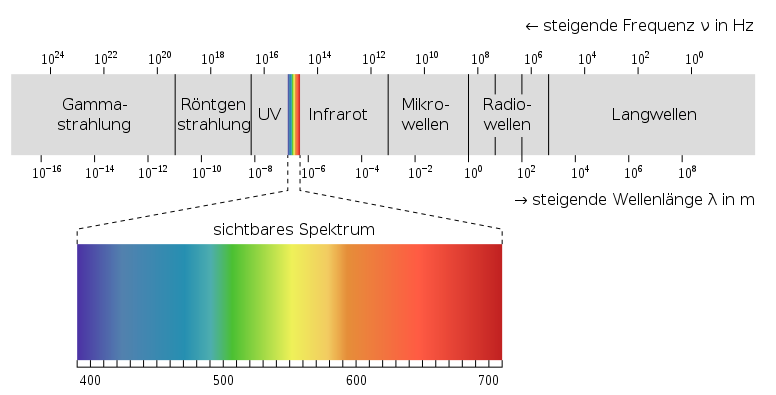
\includegraphics[width=12cm]{Bilder/emspekt.PNG}
    \end{center}
    \caption{Elekromagnetisches Spektrum}
    %\label{fig:meine-grafik}
   \end{figure}
\begin{itemize}
    \item Gammastrahlug: Gammastrahlug entsteht bei einem radioaktiven Gammazerfall. Man setzt sie
    im medizinischen Bereich ein, beispielsweise in der Strahlungstheraphie. Die hochenergetische Strahlung zerstört wucherndes Krebsgewebe indem es die entsprechende DNA zerstört. Sie
    kann nachgewiesen werden in einer Nebenkammer oder einem Geiger-Müller-Zählrohr.
    \item Röntgenstrahlung: Sie wird im medizinischen Bereich verwendet. Außerdem kann man es zur Untersuchung von Strukturen und zur Materialprüfung verwenden. Nachgewiesen kann die Strahlung 
    in Wechselwirkung mit Materie nachgewiesen werden. Man kann beispielsweise Fotoplatten einsetzen. Die Strahlung entsteht durch das Abbremsen von sehr schnellen Elektronen.
    \item UV: Die Strahlung kann sowohl natürlich als auch technisch entstehen. Lampen die UV-Strahlung erzeugen sind beipeilsweise Quecksilberdampf- und Quarzlampen. In diesen Lampen
    entsteht das Licht durch Anregung der jeweiligen Atomen in gasförmiger Phase durch Elektronen. Beim Zurückkehren in den Grundzustand emmittiern sie UV-Strahlung. Man kann die Strahlung
    detektieren, indem man den Photoeffekt nutzt. UV wird umfangreich in der Wirtschaft eingesetzt, unter anderem zur Materialprüfung oder zum aushärten von Polymeren.
    \item Sichtbares Spektrum: Der überwiegende Teil des auf der Erde vorkommenden Lichtes ensteht natürlichvorallem in der Sonne. Man kann es mit Fotoplatten detektieren.
    \item Infrarot: Es existieren Dioden, welche im Infrarotbereich abstrahlen. Man verwendet sie sehr oft bei Fernebedienungen. Infrar kann man mit thermischen Detektoren nachweisen.
    \item Mikrowellen: Mikrowellen entstehen in Laufzeitröhren oder Magnetrons. Die bekannteste technische Anwendung ist die Mikrowelle. Detektieren kann man sie mit einem Mikrowellenmessgerät.
    \item Radiowellen: Diese enstehen auf Radiosendemasten. Dort werden sie von Dipolenantennen erzeugt. Detektieren kann man sie mit einer passenden Antenne und einem Spannungsmessgerät.
    \item Langwellen: Auch diese können in der Natur vorkommen. Detektieren kann man sie mit einer passenden Antenne, hier vermutlich ein sehr langes Kabel und einem Spannungsmessgerät. 
\end{itemize} 
% Charlotte Geiger - Manuel Lippert - Leonard Schatt
% Physikalisches Praktikum

% Teilaufgabe 2

\section{Trägheitstensor $\mathbf{J}$}
% Charlotte Geiger - Manuel Lippert - Leonard Schatt
% Physikalisches Praktikum

% Teilaufgabe 3

\section{Trägheitstensor $\underline{J}_{Rad}$ eines Rades}
\label{sec: Rad}

Ist ein Rad bei der Rotation um seine Symmetrieachse ausgewuchtet nimmt der Trägheitstensor $\underline{J}_{Rad}$ im Schwerpunkt des Rades die Form einer Diagonalmatrix an. Dabei sind die Diagonalelemente wie in Kapitel \ref{sec: Traegheitstensor} erwähnt die Trägheitsmomente des Rades bei Drehung um seine Hauptachsen bzw. Symmetrieachsen. \\
Ist das Rad bei gleichartiger Bewegung nicht ausgewuchtet, ist der Trägheitstensor $\underline{J}_{Rad}$ nicht immer diagonalisierbar, d.h der Tensor hat nicht mehr die Form einer Diagonalmatrix. Diese Formänderung des Tensors wird durch zusätzliche Drehmomente, welche auf das Rad wirken, verursacht und beeinflussen das Rad bei seiner Bewegung um die Symmetrieachse. \\
Dies hat zur Folge, dass ein ausgewuchtetes Rad \enquote{rund} läuft und ein unausgewuchtetes Rad \enquote{eiert} (unregelmäßiges rotieren).
% Charlotte Geiger - Manuel Lippert - Leonard Schatt
% Physikalisches Praktikum

% Teilaufgabe 4

\section{Lage der Achsen bei Nutation eines momentfreien Kreisels}

Bei einem momentfreien Kreisel ist die Drehimpulsachse fest im Raum. Diese wird umschlossen von dem sogenannten \dq Raspolkegel\dq{}, welcher auch fest im Raum steht. Die Figurenachse bewegt sich mit der Nutationswinkelgeschwindigkeit $w_n$ um den Nutationskegel. Dabei ist die Figurenachse von dem sogenannten \dq Gangpolkegel\dq{} umschlossen, welcher sich auf dem Raspolkegel \dq abrollt\dq{} und somit den Nutationskegel entstehen lässt. Weiterhin ist die relative Lage des Raspolkegels und des Gangpolkegels zueinander festgelegt durch das Trägheitsmoment bzgl der Drehimpulsachse. % Grafik ref
% Charlotte Geiger - Manuel Lippert - Leonard Schatt
% Physikalisches Praktikum

% Teilaufgabe X

\section{Teilaufgabe 5}
% Charlotte Geiger - Manuel Lippert - Leonard Schatt
% Physikalisches Praktikum

% Teilaufgabe X

\section{Teilaufgabe 6}
Um eine Faltung zu berechnen gibt es mehrere Möglichkeiten. Ein Lösung ist es den Faltungsatz zu verwenden. Dieser besagt, dass bei Funktionen $f$ und $g$ im Ortsraum mit den 
zugehörigen Funktionen $\tilde{f}$ und $\tilde{g}$ im Fourierraum gilt:
\begin{equation}  \label{faltungssatz}
    f\ast g = \mathfrak{F}^{-1}(\tilde{f} \cdot \tilde{g}  ) = g \ast f
\end{equation}
Dieses Vorgehen ist aber manchmal etwas umständlich. In einfacheren Fällen wie diesem hier ist eine graphischen Lösung einfacher. 
Bei dieser Zeichet man die Graphen beider Funktionen. Dann spiegelt man den zu verknüfenden Graphen an der y-Achse und "schiebt" diesen dann über den ersten Graphen. 
Die Fläche die sie sich überschneiden ist dann die Funktion $f \ast g $.\\
In diesem Fall nehmen wir zwei Rechtecksfuntionen mit Höhe eins und Breite $a$ bei Rechteck 1 und $b$ bei Rechteck 2. Die beiden Rechtecke sind Achsensymetrisch bezüglisch der y-Achse.
\begin{figure}[htb]
    \centering
        \begin{minipage}[t]{0.45\linewidth}
            \centering
            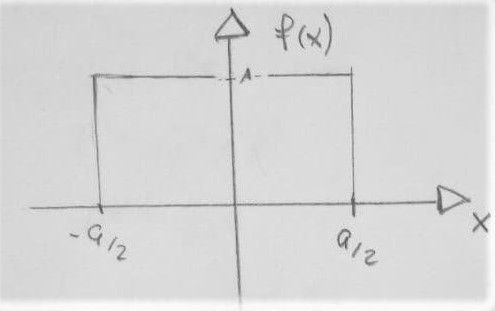
\includegraphics[width=4cm]{Bilder/FzV/frage6_1.jpg}
            \caption{Skizze von $f$}
        \end{minipage}
        \hfill
        \begin{minipage}[t]{0.45\linewidth}
            \centering
            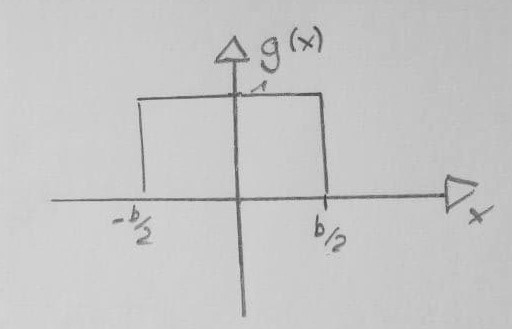
\includegraphics[width=4cm]{Bilder/FzV/frage6_2.jpg}
            \caption{Skizze von $g$}
        \end{minipage}
   
    
    %\label{fig:meine-grafik}
   \end{figure}
   Jetzt können zwei Fälle Auftreten:\\
   \begin{itemize}
       \item Fall 1: $a=b$
 
            In diesem Fall entsteht ein perfektes Dreieck, da nur in einem Punkt die volle Fläche erreicht ist.
            \begin{figure}[h]
                \centering
                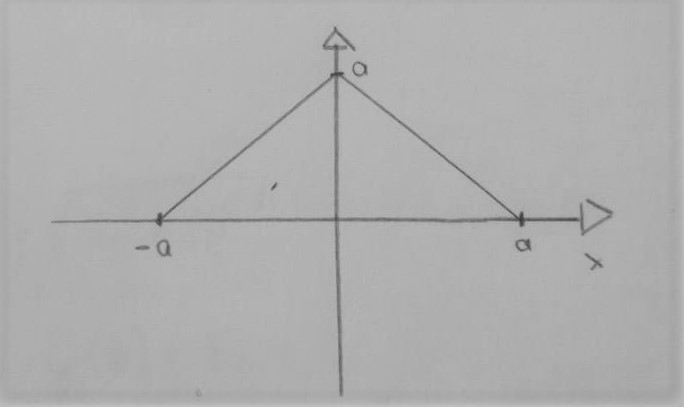
\includegraphics[width = 4cm]{Bilder/FzV/frage6_3.jpg}
                \caption{Skizze von $f \ast g$ mit $a=b$}
                \label{faltung}
            \end{figure}
        Die maximale Überschneidung der beiden Graphen ist daher $a \cdot 1 = a$.
       \item Fall 2: $a'  > b'$
            Diesmal sind die beiden Dreieck nicht Deckungsgleich. Deshalb ist die maximale Überschneidung hier nur $b' \cdot 1 = b'$. 
            Es ist also kein Dreieck wie in Abbildung \ref{faltung}, sondern dem Dreieck wurde seine Spitze abgeschnitten. 
            \newpage
            \begin{figure}[h]
                \centering
                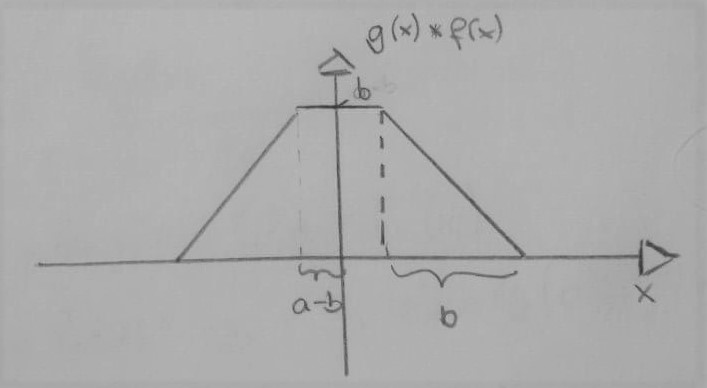
\includegraphics[width = 4cm]{Bilder/FzV/frage6_4.jpg}
                \caption{Skizze von $f\ast g$ mit $b < a$}
            \end{figure}
        \item Fall 3: $a''< b''$
            Dieser Fall ist identsich zu Fall zwei, da man O.b.d.A. $a''$ und $b''$ vertauschen kann laut Gleichung \ref{faltungssatz}.
            Das heißt, in diesem Fall erhält man wieder ein angeflachtes Dreieck.
   \end{itemize}

% Charlotte Geiger - Manuel Lippert - Leonard Schatt
% Physikalisches Praktikum

% Teilaufgabe 7

\section{Senkrechte Ausrichtung eines rotierenden Bierfilzes}
Wird ein Bierfilz, welcher um seine Figurenachse rotiert, in die Luft geworfen, erfährt dieser ein Drehmoment. Dieses wird verursacht durch die Kraftwirkung des Luftwiderstand auf den Anteil der Fläche des Bierfilz, welche senkrecht zur Luftströmung steht. Dieser Umstand hat die Folge, dass sich der Drehimpuls des Bierfilzes ändert und sich dieser damit kippt bis die Richtung des Drehimpulses senkrecht zur Strömungrichtung der Luft steht. Dabei hat der Bierfilz in dieser Position ein Minimum an Reibung durch die Luft, wodurch kein weiteres Drehmoment auf den Bierfilz ausgewirkt wird und damit die Bewegung sich stabilisiert.\\
Bei einem Diskus ändert sich dieser Vorgang, da dieser ein sehr großes Trägheitsmoment bzgl. seiner Figurenachse aufweißt, was durch seine Konstruktion (Hauptmasse möglichst weit von der Figurenachse entfernt) bedingt ist. Durch diese Konstruktion muss auf einen Diskus hohe Drehmomente wirken, damit dieser seine Ausrichtung ändert. Die von der Luftströmung verursachten Drehmomente sind dafür aber zu schwach um eine signifikante Änderung zu verursachen, bevor der Diskus auf dem Boden aufschlägt.

% etc.

    % 3.Kapitel Protokoll
    % Charlotte Geiger - Manuel Lippert - Leonard Schatt
% Physikalisches Praktikum

% 3.Kapitel  Protokoll

% Variables
\def\skalierung{0.65}

\chapter{Messprotokoll}
\label{chap:protokoll}

Das Messprotokoll wurde am Versuchstag handschriftlich erstellt und hier als
PDF-Datei eingefügt. Dabei wurden Durchführung und Aufbau schon vorher in dieses
Dokument beschrieben, je nachdem. test

%\centering

% Einbindung des Protokolls als pdf (mit Seitenzahl etc.)
% Erste Seite mit Überschrift
%\includepdf[pages = 1, landscape = false, nup = 1x1, scale = \skalierung , pagecommand={\thispagestyle{empty}\chapter{Protokoll}}]
%            {03 Protokoll/Protokoll.pdf}
% Restliche Seiten richtig skaliert
\includepdf[pages = 2-, landscape = false, nup = 1x1, scale = \skalierung , pagecommand={}]
            {03-Protokoll/ProtokollSP.pdf}

    % 4.Kapitel Versuchsauswertung
    % 4. Versuchsauswertung

\chapter{Auswertung und Diskussion}
\label{chap:versuchsauswertung}

% Text

% Input der Teilauswertung je nach Produktion der Nebendateien ohne Ordner
% Teilauswertung X

\section{Teilauswertung X}
% Teilauswertung 4
\section{Lebenszeitmessung}
\label{sec:lebenszeit}

CFP1-c1 5.008 2.9295095907141993 \\
CFP2-c1 5.008 2.86328777266995 \\
CFP3-c1 5.008 2.864972335683961 \\
YFP1-c2 5.008 3.25925836091248 \\
YFP2-c2 5.008 3.4119299746334164 \\
YFP3-c2 5.008 3.3295197646160584 \\

% etc.

    % 5.Kapitel Fazit
    % Charlotte Geiger - Manuel Lippert - Leonard Schatt
% Physikalisches Praktikum

% 5. Kapitel Einleitung

\chapter{Fazit}
\label{chap:fazit}

% Platz für Text

    % Anhang
    \chapter{Peaks für den Depolarisationsgrad}
\begin{figure}[h]
  \centering
  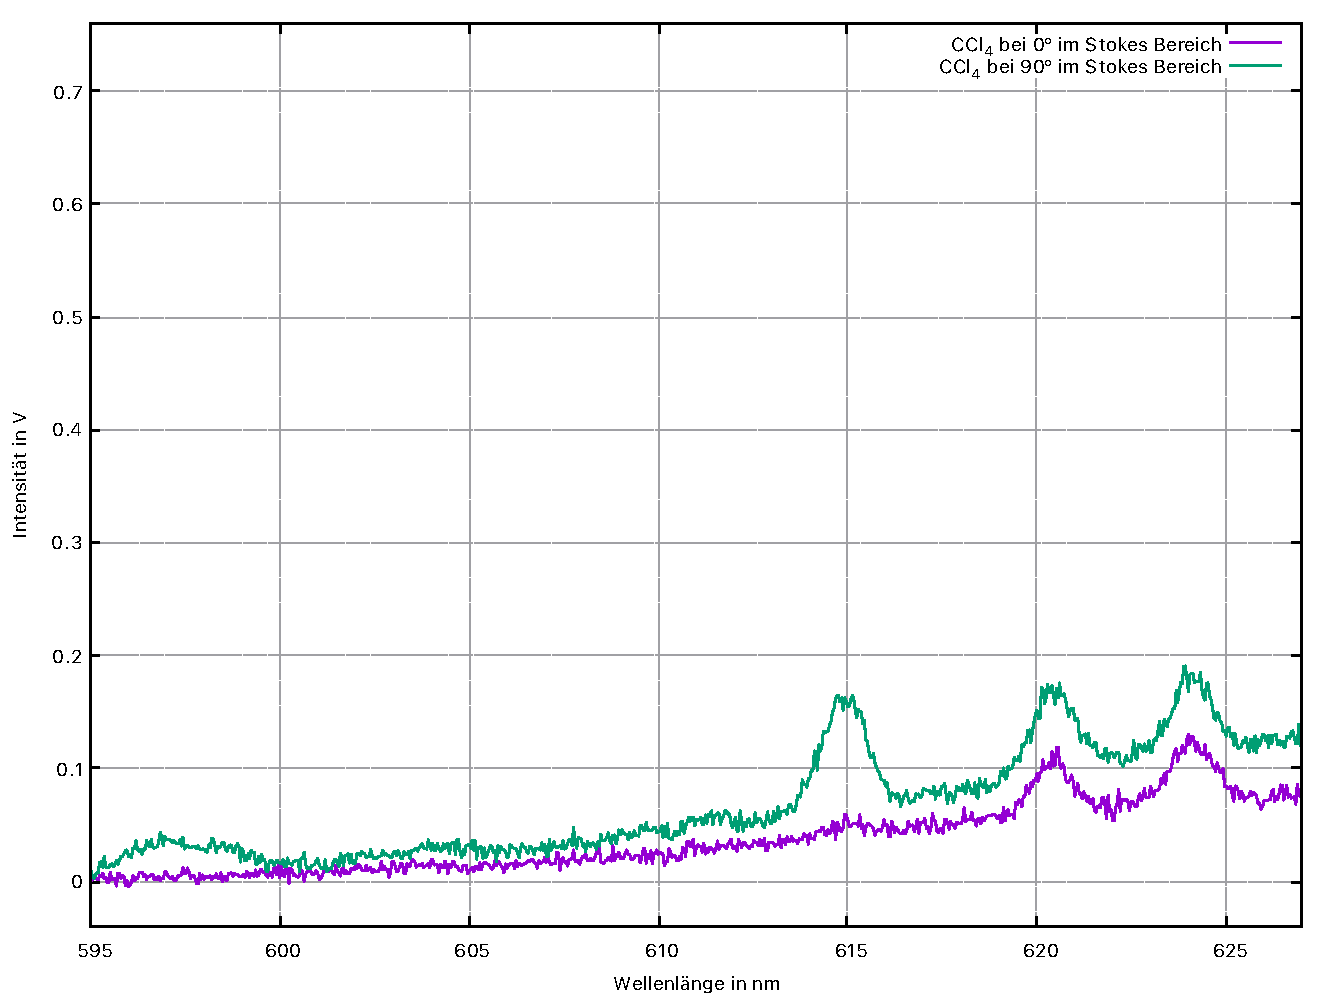
\includegraphics[scale=0.45]{Bilder/Verbesserung_Auswertung/ccl4_stokes.pdf}
  \caption{Spektrum von $CCl_4$, im Stokes Bereich bei 0° und 90° Polarisation.}
\end{figure}
\begin{figure}[h]
  \centering
  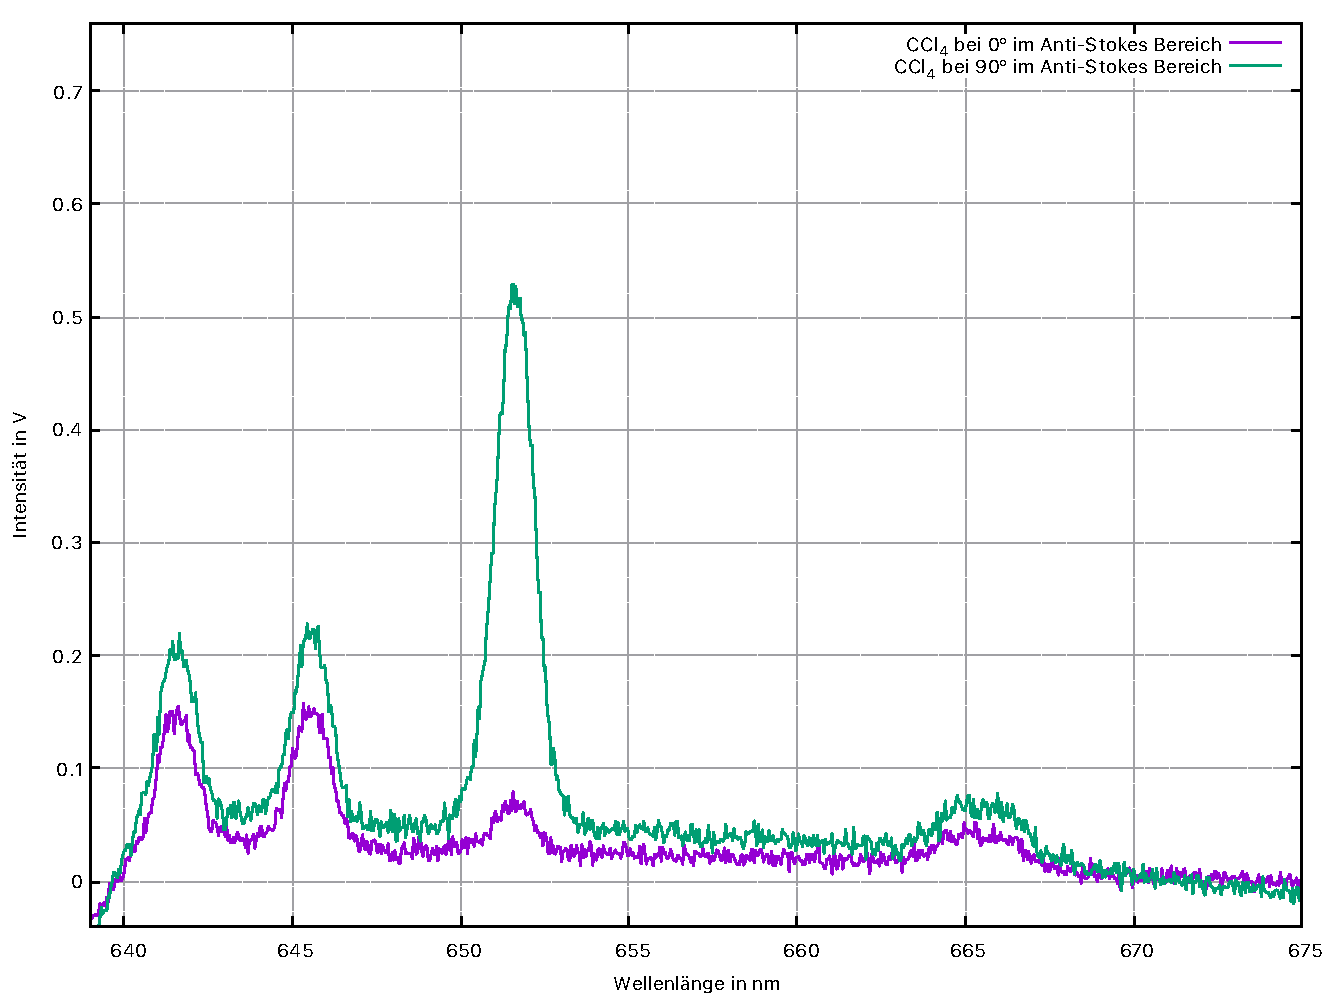
\includegraphics[scale=0.45]{Bilder/Verbesserung_Auswertung/ccl4_anti.pdf}
  \caption{Spektrum von $CCl_4$, im Anti-Stokes Bereich bei 0° und 90° Polarisation.}
\end{figure}
\begin{figure}[h]
  \centering
  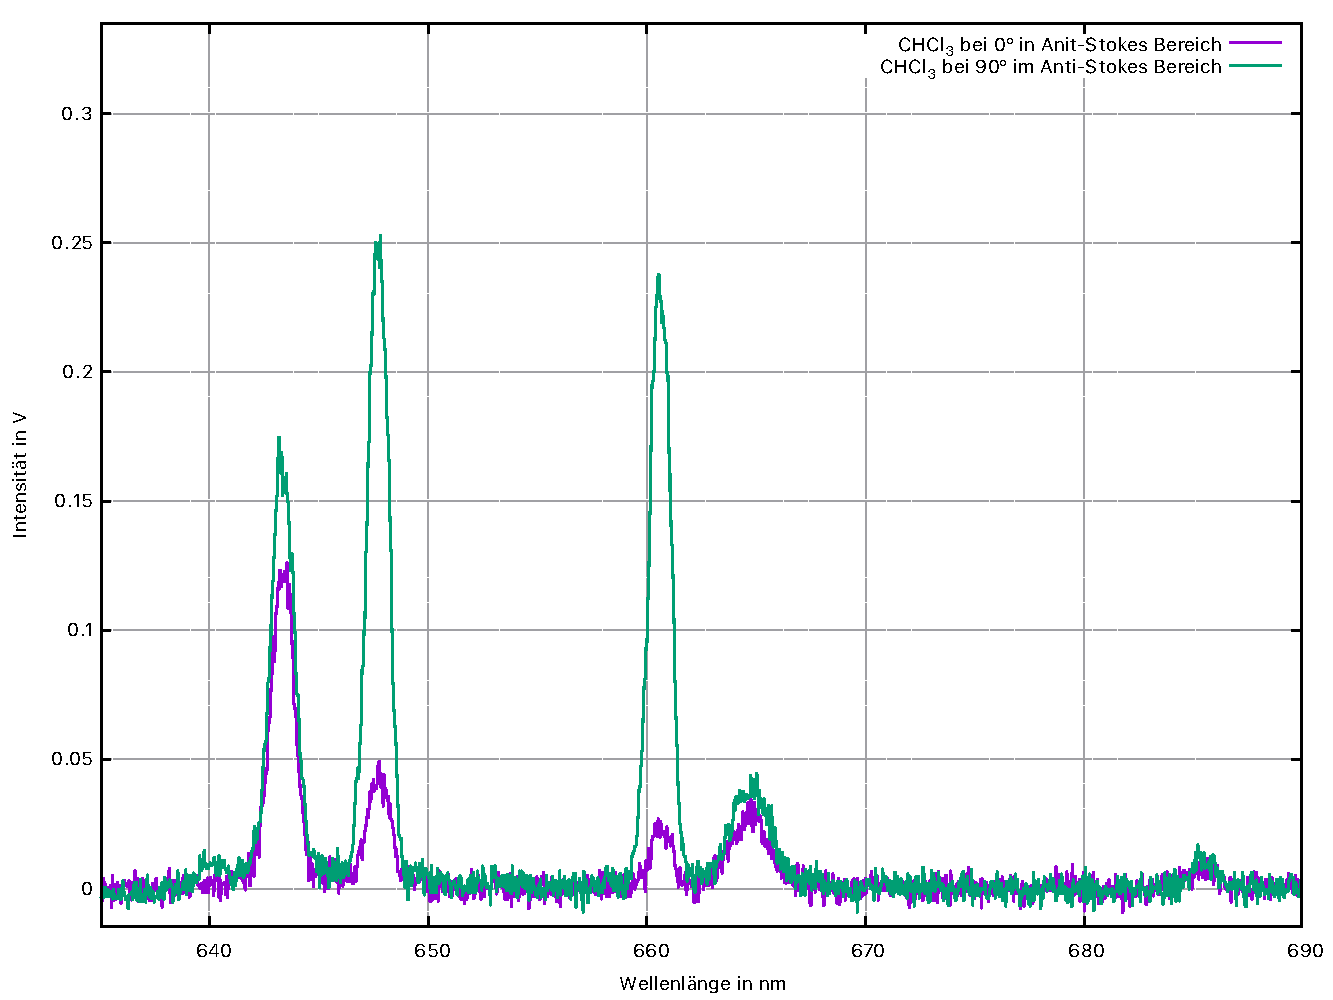
\includegraphics[scale=0.5]{Bilder/Verbesserung_Auswertung/chcl3_anti.pdf}
  \caption{Spektrum von $CHCl_3$, im Anti-Stokes Bereich bei 0° und 90° Polarisation.}
\end{figure}
\begin{figure}[h]
  \centering
  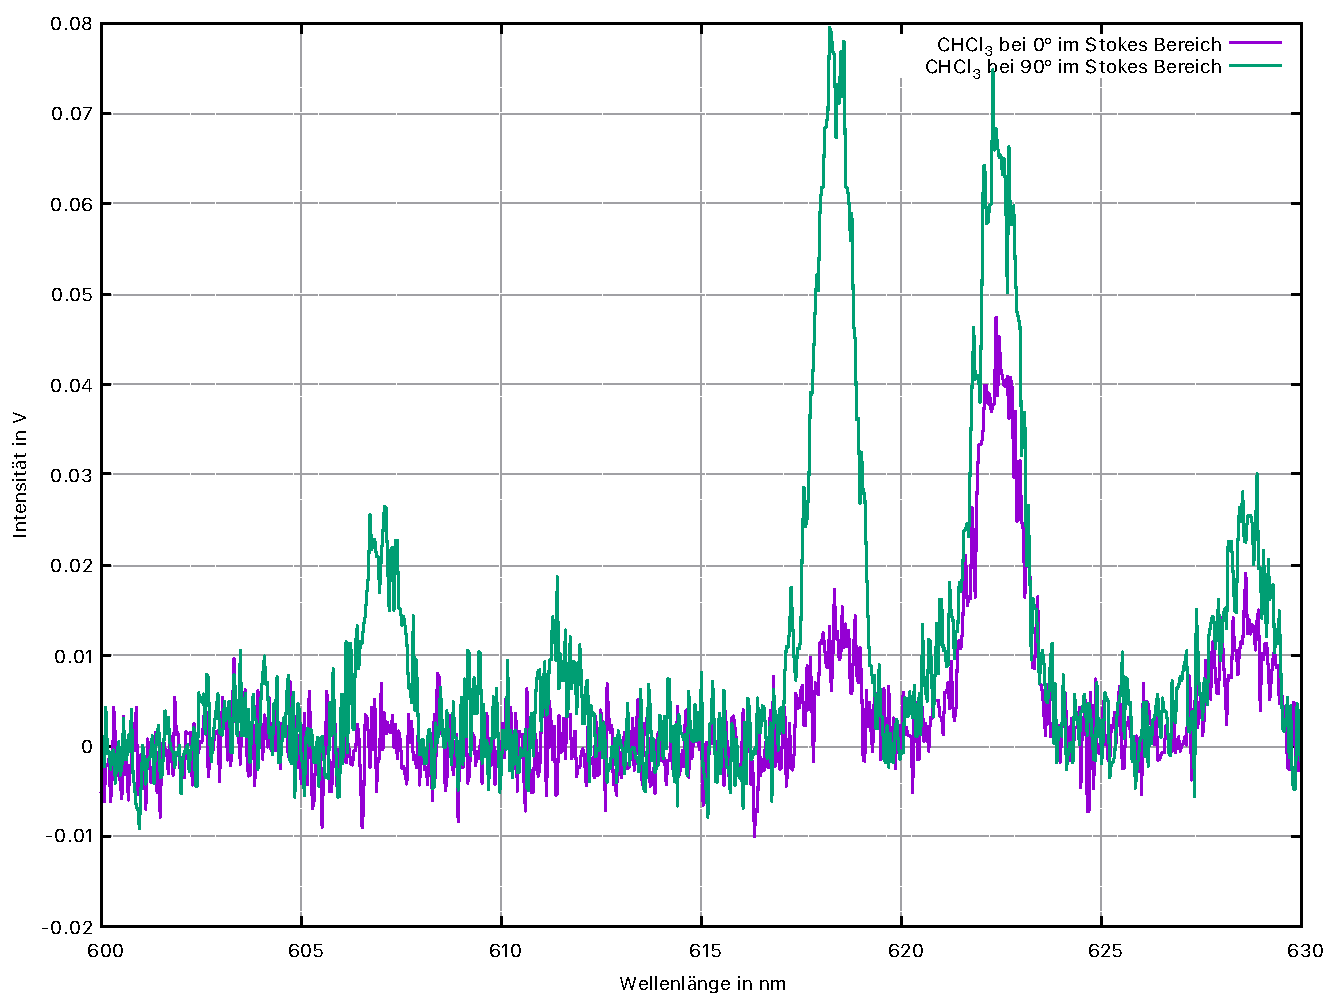
\includegraphics[scale=0.5]{Bilder/Verbesserung_Auswertung/chcl3_stokes.pdf}
  \caption{Spektrum von $CHCl_3$, im Stokes Bereich bei 0° und 90° Polarisation. In dem Bereich, indem es zur Überschneidung in der Wellenlänge bei den Peaks sowohl bei 0° als auch bei 90° kommt.}
\end{figure}

\chapter{Werte für Lage der Raman-Linien}
\begin{table}[h]
    \centering
    \begin{tabular}{c||c|c|c|c|c|c|c}
      \makecell{ $\lambda$ \\in nm} & $\nu$ in $\frac{1}{\text{cm}}$  & \makecell{ Fehler \\ $s_{\nu}$ in $\frac{1}{\text{cm}}$} & \makecell{Intensität\\ $0^{\circ}$ in V}  &  \makecell{Intensität\\ $90^{\circ}$ in V}  & \makecell{ Depolarisations- \\ grad $\rho$}  & \makecell{ Fehler \\ Depol. $s_{\rho}$} & Polarisation \\
      \hline
      643,3 & 270,4 & 12,1  & 0,1210 & 0,1688 & 0,7171 & 0,0365 & Depol. \\
      647,7 & 376,0 & 11,9  & 0,0470 & 0,2499 & 0,1879 & 0,0204 & Pol. \\
      660,7 & 679,8 & 11,5  & 0,0218 & 0,2279 & 0,0958 & 0,0220 & Pol. \\
      664,9 & 775,4 & 11,3  & 0,0281 & 0,0346 & 0,8123 & 0,1861 & Depol. \\
      685,3 & 1223,1 & 10,7  & 0,0088 & 0,0138 & 0,6359 & 0,4287 & Depol. \\  
    \end{tabular}
    \caption{Wellenlänge, Wellenzahl, Fehler der Wellenzahl, Intensität für 90° und 0°, Depolarisationsgrad und Fehler des Depolarisationsgrad für $CHCl_3$ im Anti-Stokes-Bereich.}
\end{table}
\begin{table}[h]
    \centering
    \begin{tabular}{c||c|c|c|c|c|c|c}
      \makecell{ $\lambda$ \\in nm} & $\nu$ in $\frac{1}{\text{cm}}$  & \makecell{ Fehler \\ $s_{\nu}$ in $\frac{1}{\text{cm}}$} & \makecell{Intensität\\ $0^{\circ}$ in V}  &  \makecell{Intensität\\ $90^{\circ}$ in V}  & \makecell{ Depolarisations- \\ grad $\rho$}  & \makecell{ Fehler \\ Depol. $s_{\rho}$} & Polarisation \\
    \hline
    643,3 & 270,4 & 12,1  & 0,1059 & 0,1747 & 0,6063 & 0,0335 & Depol. \\
    647,7 & 376,0 & 11,9  & 0,0434 & 0,2581 & 0,1681 & 0,0196 & Pol. \\
    659,9 & 661,5 & 11,5  & 0,0274 & 0,2651 & 0,1033 & 0,0190 & Pol. \\
    663,7 & 748,2 & 11,4  & 0,0320 & 0,0474 & 0,6754 & 0,1272 & Depol. \\
    671,4 & 921,0 & 11,1  & 0,0092 & 0,0181 & 0,5082 & 0,3092 & Depol. \\
  \end{tabular}%
\caption{Wellenlänge, Wellenzahl, Fehler der Wellenzahl, Intensität für 90° und 0°, Depolarisationsgrad und Fehler des Depolarisationsgrad für $CDCl_3$ im Anti-Stokes-Bereich.}
\end{table}\newpage
\begin{table}[h]
    \centering
    \begin{tabular}{c||c|c|c|c|c|c|c}
      \makecell{ $\lambda$ \\in nm} & $\nu$ in $\frac{1}{\text{cm}}$  & \makecell{ Fehler \\ $s_{\nu}$ in $\frac{1}{\text{cm}}$} & \makecell{Intensität\\ $0^{\circ}$ in V}  &  \makecell{Intensität\\ $90^{\circ}$ in V}  & \makecell{ Depolarisations- \\ grad $\rho$}  & \makecell{ Fehler \\ Depol. $s_{\rho}$} & Polarisation \\
      \hline
      639,0 & 165,8 & 12,3  & 0,0345 & 0,0655 & 0,5274 & 0,0863 & Depol. \\
      641,7 & 231,7 & 12,2  & 0,1201 & 0,7271 & 0,1652 & 0,0070 & Pol. \\
      655,1 & 550,4 & 11,7  & 0,0409 & 0,3626 & 0,1127 & 0,0139 & Pol. \\
      660,1 & 666,1 & 11,5  & 0,0841 & 0,1200 & 0,7007 & 0,0509 & Depol. \\  
    \end{tabular}%
    \caption{Wellenlänge, Wellenzahl, Fehler der Wellenzahl, Intensität für 90° und 0°, Depolarisationsgrad und Fehler des Depolarisationsgrad für $CHBr_3$ im Anti-Stokes-Bereich.}
\end{table}%
\begin{table}[h]
    \centering
    \begin{tabular}{c||c|c|c|c|c|c|c}
      \makecell{ $\lambda$ \\in nm} & $\nu$ in $\frac{1}{\text{cm}}$  & \makecell{ Fehler \\ $s_{\nu}$ in $\frac{1}{\text{cm}}$} & \makecell{Intensität\\ $0^{\circ}$ in V}  &  \makecell{Intensität\\ $90^{\circ}$ in V}  & \makecell{ Depolarisations- \\ grad $\rho$}  & \makecell{ Fehler \\ Depol. $s_{\rho}$} & Polarisation \\
      \hline
      641,5 & 226,8 & 12,2  & 0,1437 & 0,2009 & 0,7151 & 0,0306 & Depol. \\
      645,7 & 328,2 & 12,0  & 0,1472 & 0,2257 & 0,6520 & 0,0264 & Depol. \\
      651,7 & 470,8 & 11,8  & 0,0707 & 0,5163 & 0,1370 & 0,0098 & Pol. \\
      665,5 & 789,0 & 11,3  & 0,0381 & 0,0658 & 0,5793 & 0,0878 & Depol. \\  
    \end{tabular}
    \caption{Wellenlänge, Wellenzahl, Fehler der Wellenzahl, Intensität für 90° und 0°, Depolarisationsgrad und Fehler des Depolarisationsgrad für $CCl_4$ im Anti-Stokes-Bereich.}
  \end{table}%

    % Literatur
    \bibliographystyle{Auswertung.bst}
    \nocite{*}
    \bibliography{Auswertung.bib}

\end{document}